\chapter{Apresentação}
\renewcommand{\chaptername}{Apresentação}
\label{cap:apresentacao}

\section{Informações para contato}

% Insert the picture
\setlength\intextsep{-0.04\textwidth}
\begin{wrapfigure}{r}{-0.10\textwidth} 
	\centering
	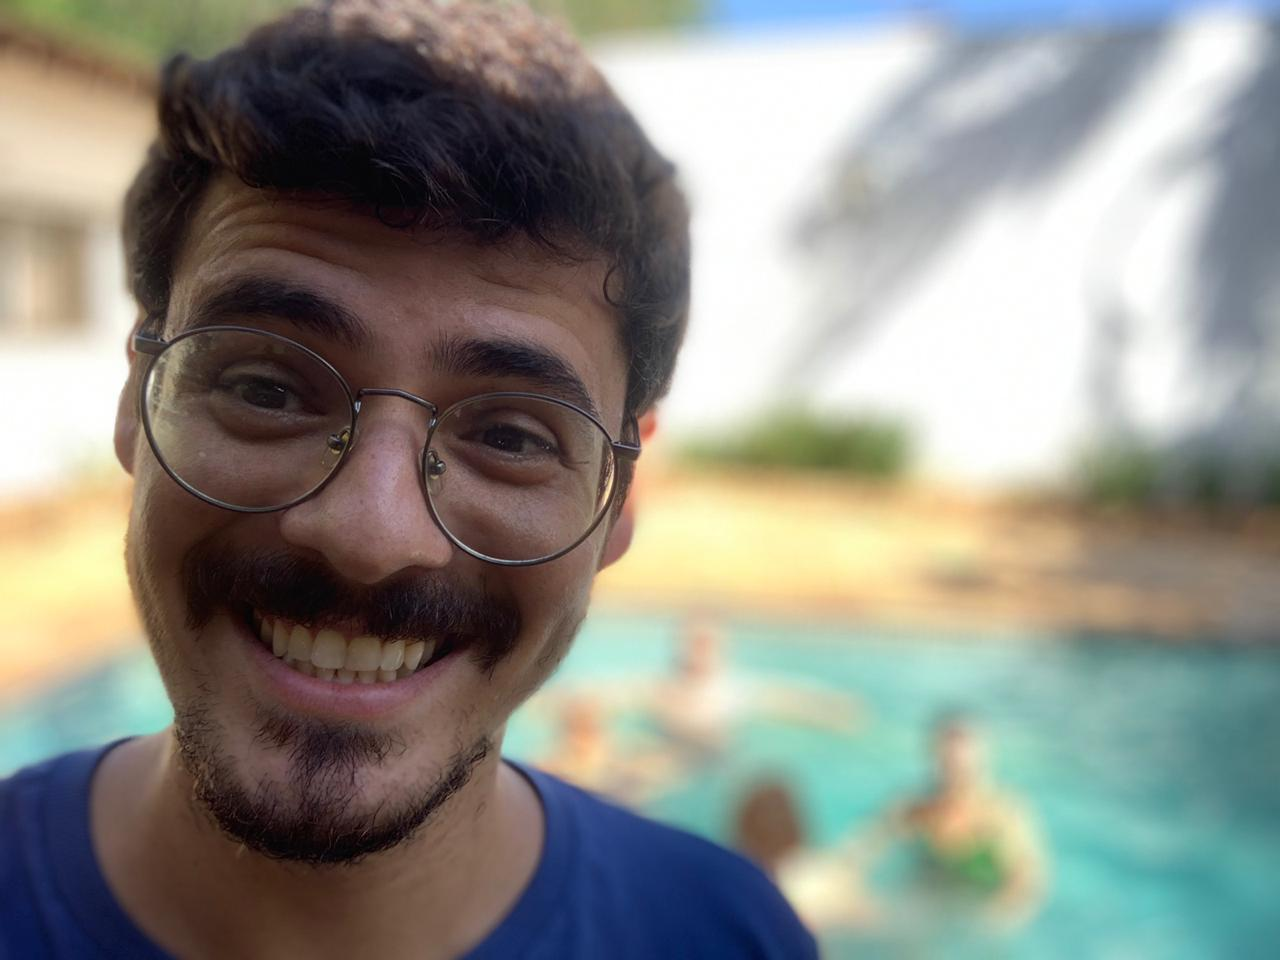
\includegraphics[width=0.42\textwidth,angle=-90]{foto.jpg}
\end{wrapfigure}

\parbox{0.03\textwidth}{\vspace{-0.1\baselineskip}\faUser} \textbf{Vanderlei C. Oliveira Jr.}\\
\parbox{0.03\textwidth}{\vspace{-0.2\baselineskip}\faUniversity} \href{https://www.gov.br/observatorio/pt-br}{\textsl{Observatório Nacional}}\\
\parbox{0.03\textwidth}{\faMapMarker} \href{https://g.page/observatorionacional?share}{\textit{Rio de Janeiro - RJ, Brasil}}\\
\parbox{0.03\textwidth}{\faEnvelope} \href{mailto:vanderlei@on.br}{\texttt{vanderlei@on.br}}\\\\
\parbox{0.03\textwidth}{\faGithub} \href{https://github.com/birocoles}{\footnotesize \texttt{github.com/birocoles}}\\
\parbox{0.03\textwidth}{\faUsers} \href{https://www.pinga-lab.org/people/oliveira-jr.html}{\footnotesize \texttt{pinga-lab.org/people/oliveira-jr}}\\
\parbox{0.03\textwidth}{\aiLattes} \href{https://lattes.cnpq.br/4332841435949533}{\footnotesize \texttt{lattes.cnpq.br/4332841435949533}}\\
\parbox{0.03\textwidth}{\aiOrcid} \href{https://orcid.org/0000-0002-6338-4086}{\footnotesize \texttt{orcid.org/0000-0002-6338-4086}}\\
\parbox{0.03\textwidth}{\aiPublonsSquare} \href{https://publons.com/researcher/1454914/oliveira-jr-v-c/}{\footnotesize  \texttt{publons.com/researcher/1454914/oliveira-jr-v-c}}\\
\parbox{0.03\textwidth}{\aiImpactstory} \href{https://impactstory.org/u/0000-0002-6338-4086}{\footnotesize \texttt{impactstory.org/u/0000-0002-6338-4086}}\\
\parbox{0.03\textwidth}{\aiResearchGateSquare} \href{https://www.researchgate.net/profile/Vanderlei-Oliveira-Jr}{\footnotesize \texttt{researchgate.net/profile/Vanderlei-Oliveira-Jr}}\\
\parbox{0.03\textwidth}{\aiFigshare} \href{https://figshare.com/authors/Vanderlei_C_Oliveira_Jr/387579}{\footnotesize \texttt{figshare.com/authors/Vanderlei{\_}C{\_}Oliveira{\_}Jr}}


\section{Formação acadêmica}


\noindent{\parbox{0.03\textwidth}{\vspace{-0.2\baselineskip}\faUserGraduate}} \textbf{\large Doutorado em Geof{\'i}sica} \\
\noindent{\parbox{0.03\textwidth}{\vspace{-0.2\baselineskip}\faUniversity}} \href{https://www.gov.br/observatorio/pt-br}{\textsl{Observat\'{o}rio Nacional}} \\
\noindent{\parbox{0.03\textwidth}{\vspace{-0.2\baselineskip}\faCalendarCheck[regular]}} Dez/2010 -- Jan/2013 \vspace{0.3\baselineskip} \\
%\parbox{0.03\textwidth}{\vspace{-0.2\baselineskip}\faUniversity} \href{https://www.gov.br/observatorio/pt-br}{\textsl{Observat\'{o}rio Nacional, Brasil}}\vspace{0.3\baselineskip} \\
%\parbox{0.03\textwidth}{\vspace{-0.2\baselineskip}\faHourglassStart}Dez/2010 -- Jan/2013 \\
\noindent \textbf{Título (portugu{\^e}s):} \textit{Processamento e invers\~{a}o de dados de campos potenciais: novas abordagens} \\
\noindent \textbf{Título (ingl{\^e}s):} \textit{Processing and inversion of potential field data: new approaches} \\
\noindent \textbf{Orientadora:} \href{https://orcid.org/0000-0002-9767-6044}{Dra. Val{\'e}ria C. F. Barbosa} \\
\noindent{\parbox{0.03\textwidth}{\vspace{-0.2\baselineskip}\faInfoCircle}}
Desenvolvi duas metodologias para o 
processamento e interpretação de dados gravimétricos e magnetométricos. A primeira é
a \textit{Camada Equivalente Polinomial} (\textit{Polynomial Equivalent Layer}), que 
é uma metodologia computacionalmente eficiente para processar grandes volumes de dados 
via t{\'e}cnica da camada equivalente. A segunda {\'e} uma metodologia para estimar a
geometria de corpos 3D isolados via inversão não-linear de dados de gradiometria da gravidade. \\
\noindent \texttt{\textbf{doi:}}  \href{https://doi.org/10.6084/m9.figshare.20334651.v1}{\texttt{ 10.6084/m9.figshare.20334651.v1}} \\

\clearpage

\noindent{\parbox{0.03\textwidth}{\vspace{-0.2\baselineskip}\faUserGraduate}} \textbf{\large Mestrado em Geof{\'i}sica} \\
\noindent{\parbox{0.03\textwidth}{\vspace{-0.2\baselineskip}\faUniversity}} \href{https://www.gov.br/observatorio/pt-br}{\textsl{Observat\'{o}rio Nacional, Brasil}} \\ \noindent{\parbox{0.03\textwidth}{\vspace{-0.2\baselineskip}\faCalendarCheck[regular]}} Mar/2009 -- Nov/2010 \vspace{0.3\baselineskip} \\
\noindent \textbf{Título (português):} \textit{Invers\~{a}o gravim\'{e}trica radial por camadas para a reconstru\c{c}\~{a}o de corpos geol\'{o}gicos 3D} \\
\noindent \textbf{Título (inglês):} \textit{Radial gravity inversion by layers for retrieving 3D geological bodies} \\
\noindent \textbf{Orientadora:} \href{https://orcid.org/0000-0002-9767-6044}{Dr. Val{\'e}ria C. F. Barbosa} \\
\noindent\noindent{\parbox{0.03\textwidth}{\vspace{-0.2\baselineskip}\faInfoCircle}}
Desenvolvi uma metodologia para
estimar a geometria de um corpo geol{\'o}gico 3D via invers{\~a}o n{\~a}o-linear 
de dados gravimétricos. \\
\noindent \texttt{\textbf{doi:}} \href{https://doi.org/10.6084/m9.figshare.20334531.v1}{ \texttt{10.6084/m9.figshare.20334531.v1}} \\

\medskip

\noindent{\parbox{0.03\textwidth}{\vspace{-0.2\baselineskip}\faUserGraduate}} \textbf{\large Bacharelado em Geof{\'i}sica} \\
\noindent{\parbox{0.03\textwidth}{\vspace{-0.2\baselineskip}\faUniversity}} \href{https://www.iag.usp.br/international/}{\textsl{Universidade de S\~{a}o Paulo, Brasil}} \\
\noindent{\parbox{0.03\textwidth}{\vspace{-0.2\baselineskip}\faCalendarCheck[regular]}} Mar/2004 -- Dez/2008 \vspace{0.3\baselineskip} \\
\noindent \textbf{T{\'i}tulo (portugu{\^e}s):} \textit{Modelagem gravim\'{e}trica 3D da borda norte da Bacia do Paran\'{a}} \\
\noindent \textbf{T{\'i}tulo (ingl{\^e}s):} \textit{3D gravity modelling of the northern border of the Paran\'{a} basin} \\
\noindent \textbf{Orientadora:} \href{https://orcid.org/0000-0003-4329-1787}{Dra. Y{\'a}ra R. Marangoni} \\
\noindent\noindent{\parbox{0.03\textwidth}{\vspace{-0.2\baselineskip}\faInfoCircle}}
Apliquei uma metodologia para estimar a geometria do 
embasamento e da Moho a partir da inversão não-linear de dados gravimétricos 
sobre a borda norte da Bacia do Paraná.


\section{Contextualização e considerações pessoais}
\label{sec:apresentacao-consideracoes}

Trabalho com desenvolvimento de métodos numéricos para o processamento e
interpretação de dados gravimétricos e magnetométricos desde quando comecei
a graduação em geofísica, em 2004, no IAG-USP, São Paulo.
Desde aquela época eu queria ser cientista, ainda que este conceito tenha mudado 
bastante para mim ao longo dos anos. Se por um lado essa certeza me ajudou a 
ter muito foco nas minhas decisões, por outro lado ela fez com que eu não experimentasse
o caminho da iniciativa privada. Mas acho que foi melhor assim.

\bigskip

\noindent Durante o meu curso de graduação, fiz iniciação
científica sob a supervisão da professora Dra. \href{https://lattes.cnpq.br/5050611044655332}{Y{\'a}ra R. Marangoni}. 
Foi naquela época que aprendi a programar, cursei algumas disciplinas na pós graduação e 
comecei a investigar métodos numéricos para estimar o relevo do embasamento sob uma bacia
sedimentar via inversão de dados gravimétricos. 
Durante a minha IC, acreditei ter desenvolvido um método iterativo para estimar o relevo do
embasamento. 
Em uma conversa com o Dr \href{https://lattes.cnpq.br/6171841822916587}{Wladimir Shukowsky}, contudo, ele me mostrou que meu trabalho não era novo.
De fato, ele me apresentou um artigo intitulado 
\textit{``The use of rapid digital computing methods for direct gravity interpretation of sedimentary basins''}, publicado em 1960 por M. H. P. Bott (\texttt{doi:} \href{https://doi.org/10.1111/j.1365-246X.1960.tb00065.x}{\texttt{10.1111/j.1365-246X.1960.tb00065.x}}), que contém praticamente tudo que eu pensei ter desenvolvido naquela época.
Os resultados do meu trabalho foram divulgados no seguinte resumo de congresso:
\begin{enumerate}
	\item \bibentry{sbgf_2009}
\end{enumerate}

\bigskip

\noindent No final da minha graduação, tentei ingressar no doutorado do IAG-USP mas, 
felizmente, o departamento recusou. Digo ``felizmente'' porque considero que o mestrado 
foi uma transição necessária entre a graduação e o doutorado.
A Dra. Y{\'a}ra me colocou em contato com a Dra. \href{https://lattes.cnpq.br/0391036221142471}{Valéria C. F.Barbosa}, do Observatório Nacional (ON), e eu acabei sendo aprovado (em último lugar)
no processo seletivo para o mestrado em Geofísica do ON. Lembro que além da minha
orientadora na época, a Dra. Yára, os professores 
Dr. \href{https://lattes.cnpq.br/3934334115083849}{Ricardo Trindade} e
Dr. \href{https://lattes.cnpq.br/0921576804781499}{Eder Molina} também 
me incentivaram a seguir meus estudos começando pelo mestrado.
Em Março de 2009, mudei-me para o Rio de Janeiro e comecei meu mestrado no ON sob a
supervisão da Dra. Valéria.

\bigskip

\noindent O projeto que desenvolvi durante o mestrado foi proposto pela minha orientadora e consistiu
em desenvolver uma metodologia para estimar a forma de uma fonte isolada 3D via inversão
não-linear de dados gravimétricos. Felizmente, correu tudo bem e concluí o mestrado 
em Novembro de 2010, pouco menos de dois anos após ter iniciado o curso.
Os resultados do mestrado foram divulgados em eventos científicos
\begin{enumerate}
	\item \bibentry{eage_2014}
	\item \bibentry{eage_2011}
	\item \bibentry{sbgf_2011}
	\item \bibentry{seg_2011}
\end{enumerate}
\noindent e publicados no artigo abaixo:
\begin{enumerate}
	\item \bibentry{oliveirajr_etal2011} 
\end{enumerate}

\bigskip

\noindent Logo após terminar o mestrado, em dezembro de 2010, ingressei no doutorado em Geofísica,
também sob orientação da Valéria no ON. Dessa vez, o projeto foi proposto por mim
e eu conduzi a pesquisa de forma mais independente. Uma das ideias que desenvolvi no 
doutorado foi uma continuação do meu mestrado. Essa ideia era uma metodologia para
estimar a forma de uma fonte isolada a partir da inversão não-linear de dados de 
gradiometria da gravidade. Já a outra ideia surgiu a partir de uma disciplina oferecida
pela Valéria no ON. Foi naquela disciplina que aprendi sobre a técnica da camada 
equivalente. Na época eu fiquei muito interessado nisso porque envolvia muita teoria e eu
sempre gostei de coisas teóricas.
Certo dia, em uma conversa na mesa de um bar em São Cristóvão com meu amigo Dr
\href{https://www.leouieda.com/}{Leonardo Uieda}, que também cursava a pós-graduação no ON, pensamos em reparametrizar a
distribuição de propriedade física sobre a camada equivalente em termos de um conjunto de
polinômios bivariados. Desenvolvi essa ideia como parte do meu doutorado e disso 
surgiu uma técnica computacionalmente eficiente para processamento de dados gravimétricos
e magnéticos via camada equivalente.

\bigskip

\noindent No final de 2012, bem no meio do meu doutorado, houve um concurso para pesquisador no ON.
Na época, nem eu e nem a minha orientadora nos atentamos ao fato de que eu poderia 
prestar o concurso, mesmo sem ter concluído o doutorado, que era um dos pré-requisitos do
cargo. Foi em uma das (muitas) festas dos estudantes de pós-graduação no ON que
o Dr \href{https://lattes.cnpq.br/5822763057370791}{Fernando Roig} veio me falar que eu poderia prestar o concurso.
Ele chamou a atenção para um detalhe do edital: a documentação comprobatória da conclusão 
do doutorado deveria ser apresentada na posse, portanto após o concurso. 
Ou seja, eu poderia prestar o concurso e, caso fosse aprovado, deveria defender o doutorado
o mais rápido possível para poder assumir o cargo.
Foi então que eu prestei o concurso no final de 2012, fui aprovado e defendi minha tese em
Janeiro de 2013, cerca de dois anos após ter começado o doutorado. 
Tomei posse como pesquisador
em Julho de 2013. Os resultados do meu doutorado foram divulgados em eventos científicos
\begin{enumerate}
	\item \bibentry{sbgf_2013}
	\item \bibentry{sbgf_2012}
	\item \bibentry{seg_2012}
\end{enumerate}
\noindent e publicados nos artigos abaixo:
\begin{enumerate}
	\item \bibentry{oliveirajr_barbosa2013}
	\item \bibentry{oliveirajr_etal_2013}
\end{enumerate}

\bigskip

\noindent Mais importante do que o conhecimento técnico acumulado na graduação e, 
principalmente, no mestrado e doutorado, acho que a independência acadêmica 
foi a principal lição que aprendi naquela época.
Obviamente, isso não significa que eu estava preparado para seguir a minha 
carreira completamente sozinho desde aquela época. O que quero dizer com 
independência acadêmica é que eu tinha começado a ter minhas próprias ideias
e a conseguir investigá-las de forma mais independente.
No doutorado aprendi que o pesquisador deve ser um especialista em aprender
e que o rigor científico necessário para chegar a uma determinada conclusão pode ser
mais importante do que a própria conclusão.
